% Slide 4e: screen-and-certify design loop (Study 9). Numbers are from the committed Study 9 results.
\documentclass[border=8pt]{standalone}
% Shared preamble for the slide diagrams. Palette and ink colours match figures/make_figures.py.
\usepackage[T1]{fontenc}
\usepackage{dejavu}
\renewcommand{\familydefault}{\sfdefault}
\usepackage{amsmath,amssymb}
\usepackage{xcolor}
\usepackage{tikz}
\usetikzlibrary{arrows.meta,positioning,shapes.geometric,calc,fit,backgrounds,decorations.pathmorphing,patterns}

\definecolor{surface}{HTML}{FCFCFB}
\definecolor{ink}{HTML}{0B0B0B}
\definecolor{inktwo}{HTML}{52514E}
\definecolor{muted}{HTML}{898781}
\definecolor{gridc}{HTML}{E1E0D9}
\definecolor{axisc}{HTML}{C3C2B7}
\definecolor{cblue}{HTML}{2A78D6}
\definecolor{corange}{HTML}{EB6834}
\definecolor{cgreen}{HTML}{1BAF7A}
\definecolor{camber}{HTML}{EDA100}

\newcommand{\tg}[1]{{\scriptsize\color{inktwo}#1}}  % small secondary line inside a node

\pagecolor{surface}
\color{ink}

\tikzset{
  every node/.style={text=ink},
  % one box style; the argument is the role colour (blue learned, inktwo exact/fixed, corange verification, ...)
  box/.style={draw=#1, fill=#1!10, rounded corners=3pt, line width=0.9pt, align=center,
              inner xsep=6pt, inner ysep=5pt, minimum height=1.25cm, text width=2.75cm, font=\footnotesize},
  tag/.style={font=\scriptsize, text=inktwo, align=center},
  arr/.style={-{Stealth[length=5.5pt,width=4.5pt]}, line width=0.9pt, color=inktwo},
  darr/.style={arr, dashed},
}

\begin{document}
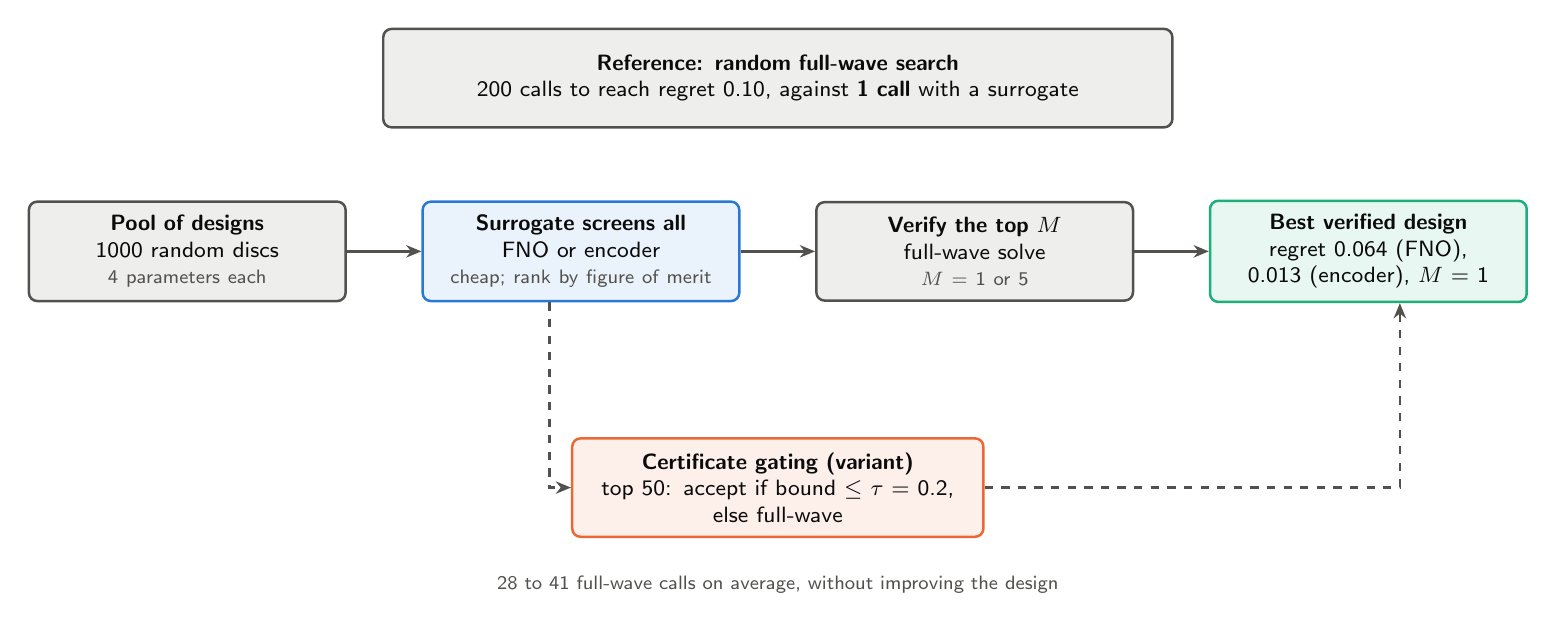
\begin{tikzpicture}[x=1cm,y=1cm, box/.append style={text width=3.6cm}]
  \node[box=inktwo]  (pool)   at (0,0)    {\textbf{Pool of designs}\\1000 random discs\\\tg{4 parameters each}};
  \node[box=cblue]   (screen) at (5.0,0)  {\textbf{Surrogate screens all}\\FNO or encoder\\\tg{cheap; rank by figure of merit}};
  \node[box=inktwo]  (top)    at (10.0,0) {\textbf{Verify the top $M$}\\full-wave solve\\\tg{$M$ = 1 or 5}};
  \node[box=cgreen]  (best)   at (15.0,0) {\textbf{Best verified design}\\regret 0.064 (FNO),\\0.013 (encoder), $M$ = 1};
  \draw[arr] (pool) -- (screen);
  \draw[arr] (screen) -- (top);
  \draw[arr] (top) -- (best);

  % certificate gating variant
  \node[box=corange, text width=4.8cm] (gate) at (7.5,-3.0)
        {\textbf{Certificate gating (variant)}\\top 50: accept if bound $\le\tau$ = 0.2,\\else full-wave};
  \draw[darr] ([xshift=-0.4cm]screen.south) |- (gate.west);
  \draw[darr] (gate.east) -| ([xshift=0.4cm]best.south);
  \node[tag, anchor=north, text width=11cm] at (7.5,-4.0)
        {28 to 41 full-wave calls on average, without improving the design};

  % comparison strip
  \node[box=inktwo, text width=9.6cm] (rand) at (7.5,2.2)
        {\textbf{Reference: random full-wave search}\\200 calls to reach regret 0.10, against \textbf{1 call} with a surrogate};
\end{tikzpicture}
\end{document}
